% !TeX root = ../thuthesis-example.tex

\chapter{API优先开发的设计与实现}
\label{chap:api-first}

API优先开发(API-First Development)是一种软件设计与开发方法论,其核心在于在实际开发前完成应用程序接口(Application Programming Interface, API)的设计与定义。明确的API规范使开发团队能在实际实现前达成共识,促进前端、后端和移动端的并行开发,减少集成阶段的冲突和重复工作。统一的API设计确保系统各服务接口的一致性,降低维护成本。以API为界面的系统设计也推动了模块化和解耦架构的形成,各服务只需关注自身API的实现和使用,无需了解其他组件的内部工作机制。

本章将介绍API优先开发在bolt.SE中的实现方案与实例应用场景。

\section{API优先开发对于bolt.SE的意义}

在LLM驱动的软件开发中,API优先方法具有独特价值。LLM与外部系统交互需要明确的结构和规范,API定义为LLM提供了调用外部服务的具体指南,减少模糊指令导致的错误。通过API集成,LLM能够获取实时数据和使用专业工具,扩展其能力范围。API定义中的认证和授权机制为LLM提供了受控的访问方式,确保其操作在安全合规的范围内执行。此外,API优先方法支持LLM将复杂任务分解为多个API调用的组合,提高问题解决效率。

bolt.SE将API优先理念融入平台设计,通过将OpenAPI规范集成到开发流程中,实现LLM与外部API的有效协作,开发者能通过自然语言交互获得API增强的开发支持。bolt.SE的APIActions模块结合了LLM的灵活性与API的精确性和功能扩展性,有效提升了软件开发效率。

\section{bolt.SE中的OpenAPI应用}

在bolt.SE的设计过程中,我们选择OpenAPI规范作为API描述标准,主要基于其广泛的行业接受度、丰富的工具生态系统以及对机器可读格式的良好支持。相比其他API描述格式,OpenAPI提供了更完整的功能描述能力和更好的扩展性,这些特性使其特别适合与LLM集成,便于模型理解和处理API结构。

OpenAPI规范(原Swagger规范)是API优先开发的主流规范之一,为API描述和交互提供了标准化、语言无关的格式\cite{openapi2023}。作为业界广泛采用的API定义标准,OpenAPI使开发者能以声明式方式完整定义API的各方面,实现从设计到实现、测试和文档的全生命周期管理。

OpenAPI规范采用JSON或YAML格式,结构化描述API的端点(endpoints)、操作(operations)、参数、响应、认证方法等关键要素。这种规范不仅适合人类理解,也便于机器处理,成为前端、后端和各类工具间沟通的桥梁。在bolt.SE的开发环境中,OpenAPI规范定义RESTful API调用说明,从而更高效地利用现有功能,避免重复开发,结构化API定义还能够避免在大模型上下文中包含冗长API使用说明,节省token空间。

OpenAPI规范主要包含以下组成部分\cite{openapi2023spec}:

\begin{enumerate}
  \item 基本信息:API的标题、描述、版本、联系人信息和许可证等元数据。
  
  \item 服务器信息:API的基础URL和不同环境(开发、测试、生产)的服务器地址。
  
  \item 路径:API的各端点及可用HTTP方法(GET、POST、PUT、DELETE等),是规范核心部分。
  
  \item 组件:包含可重用部分:
    \begin{itemize}
      \item \textit{schemas}:API使用的数据模型和对象结构。
      \item \textit{parameters}:可重用的参数定义。
      \item \textit{responses}:各种响应格式和状态码。
      \item \textit{securitySchemes}:API支持的安全认证机制。
    \end{itemize}
  
  \item 操作:每个API端点的可用操作,包括操作ID与摘要、描述与标签、参数定义(路径、查询、头部、cookie等)、请求体结构与格式、可能的响应状态与内容及所需安全机制。
\end{enumerate}

以下是bolt.SE中支持的OpenAPI定义示例,展示一个简单的天气API:

\begin{minted}{yaml}
openapi: 3.0.0
info:
  title: Weather API
  version: 1.0.0
servers:
  - url: https://api.weather.gov
    description: Weather API Server
paths:
  /weather/current:
    get:
      summary: Get current weather
      parameters:
        - name: city
          in: query
          required: true
          schema:
            type: string
      responses:
        '200':
          description: Current weather data
          content:
            application/json:
              schema:
                type: object
                properties:
                  temperature:
                    type: number
                  conditions:
                    type: string
\end{minted}

bolt.SE的APIActions模块解析这类OpenAPI定义,提取API端点和操作,使LLM能理解并正确调用这些API。

\section{bolt.SE中的APIActions实现}
bolt.SE通过APIActions模块,使用户能够定义、管理和应用外部API,同时使LLM能理解并调用这些API,实现功能扩展和技术集成。图\ref{fig:api_workflow}展示了完整的API使用工作流程,包括用户创建、编辑和使用API的流程,以及API信息在系统各组件间的传递方式。

\begin{figure}[H]
  \makebox[\textwidth][c]{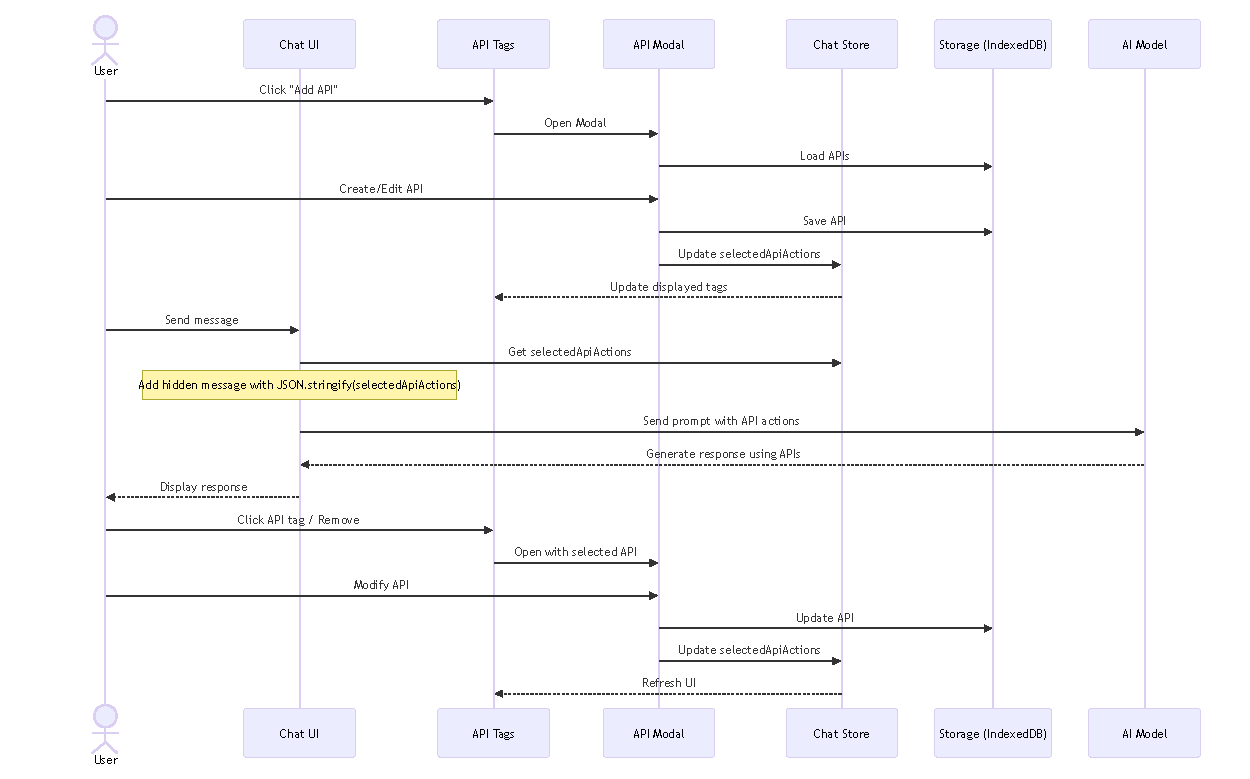
\includegraphics[width=1.2\textwidth]{figures/api_workflow.pdf}}
  \caption{API使用工作流程图:展示用户创建、编辑和使用API的完整流程,以及API信息在系统各组件间的传递方式}
  \label{fig:api_workflow}
\end{figure}

APIActions是bolt.SE中实现API优先开发的核心功能模块,为LLM提供识别、理解和调用外部API的能力,同时优化token使用效率。该模块基于结构化数据模型设计,通过系统化的类结构定义API信息,实现从规范解析到功能调用的完整流程。图\ref{fig:api_actions_class}展示了APIActions的数据模型类图,描述了系统如何组织和管理API定义。

\begin{figure}[H]
  \centering
  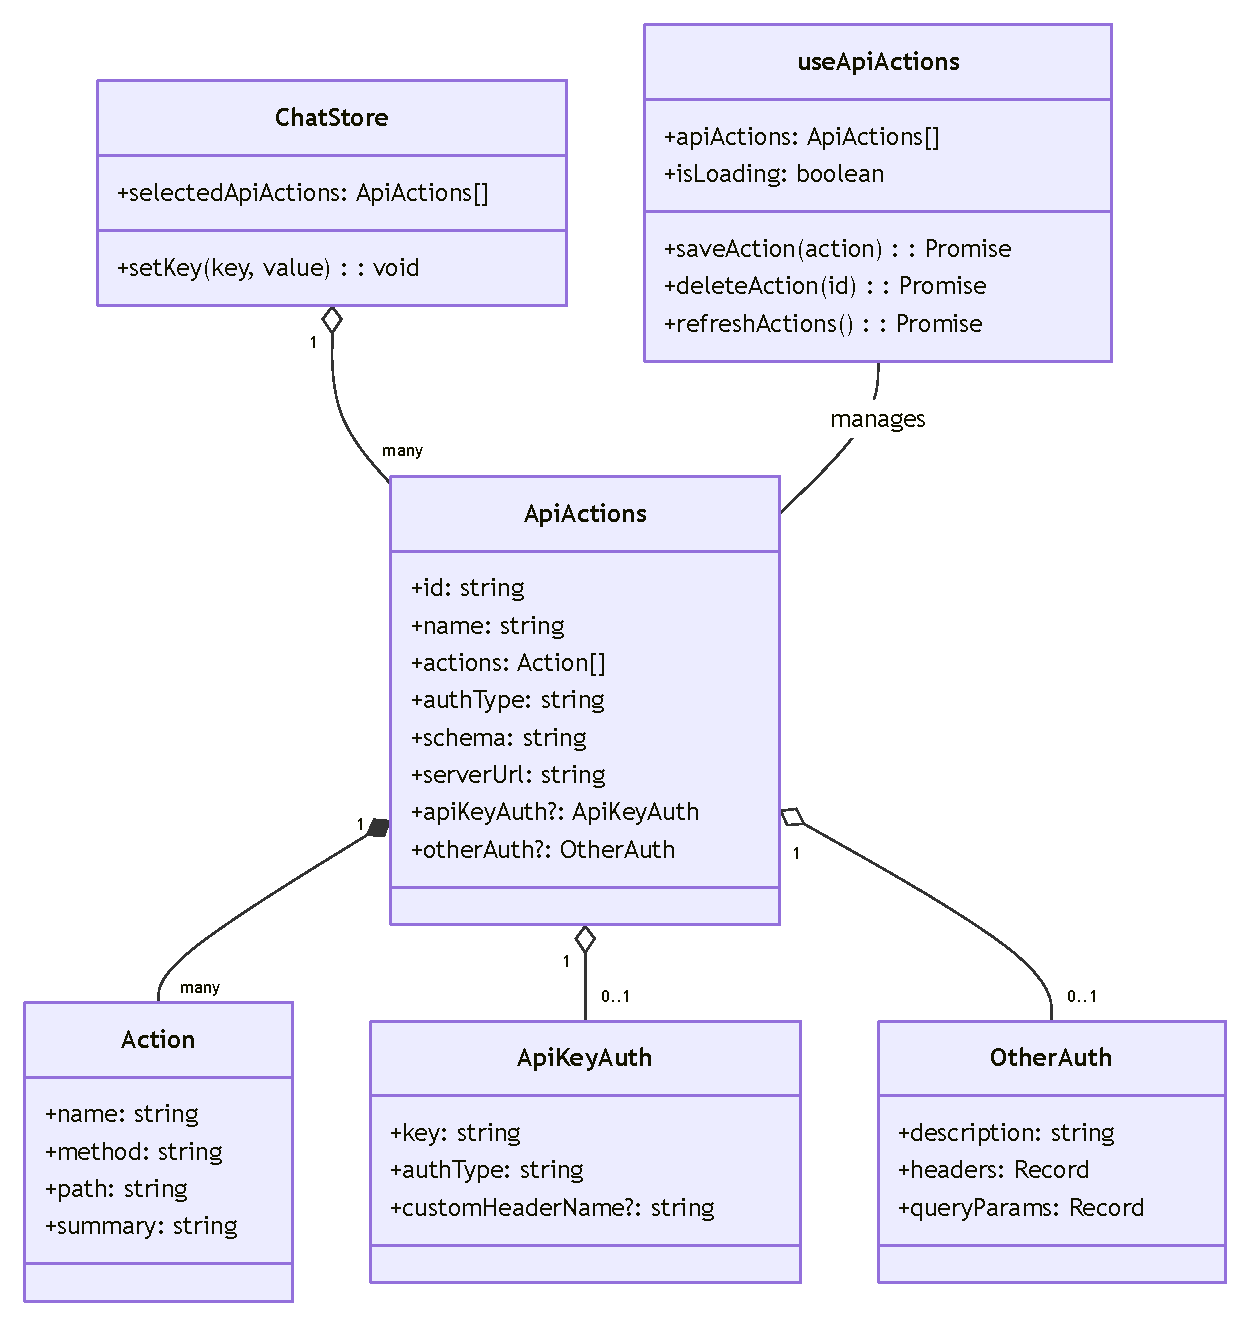
\includegraphics[width=\textwidth]{figures/api_actions_class.pdf}
  \caption{API数据模型类图:描述系统中API定义的核心数据结构及其关系,包括API操作、认证方式和存储管理}
  \label{fig:api_actions_class}
\end{figure}

ApiActions类是核心数据结构,包含API的所有必要信息:

\begin{enumerate}
  \item 基本信息:唯一标识符(id)、名称(name)和基础URL(serverUrl)。
  
  \item API操作集:由多个Action对象组成,每个Action定义一个API端点的HTTP方法、路径和功能摘要。
  
  \item 认证信息:支持无需认证的API(none)、API密钥认证(apiKey,支持Basic、Bearer或自定义头部方式)以及其他自定义认证(other,可配置自定义头部和查询参数)。
  
  \item OpenAPI规范:通过schema字段存储完整OpenAPI规范定义,为系统提供API详细信息。
\end{enumerate}

APIActions通过以下几种方式优化了LLM应用效率:

\begin{enumerate}
  \item 结构化Schema传递:将OpenAPI规范解析为紧凑的TypeScript数据模型,仅保留端点信息与参数定义的核心要素,相比原始描述节省token消耗。
  
  \item 外部数据获取:LLM能透过提供的API,直接访问实时数据源,如天气服务或金融API。
  
  \item 模块化上下文管理:用户可通过\texttt{ApiActionsContextTags}组件控制当前对话中加入哪些API定义作为上下文,避免全量API信息占用上下文窗口。
  
  \item 缓存与持久化优化:系统通过IndexedDB持久化存储API定义,避免重复传输API信息,在多轮对话中持续复用已定义的API结构,降低冗余信息传递。
  \end{enumerate}

\section{实例应用场景}

本节以聊天机器人应用为例,展示bolt.SE中APIActions模块如何集成外部API并借助LLM实现任务规划和代码生成。该机器人集成了OpenAI API、NWS Weather API与The Dog API,能够回答天气相关问题并展示狗狗图片。

\subsection{API配置与应用开发流程}

用户首先通过图形界面配置所需API(图\ref{fig:demo_edit}),粘贴OpenAPI定义并选择认证方式。配置完成后,所有API在总览界面中可见(图\ref{fig:demo_table}),支持编辑、删除和重载操作。用户在主对话框中勾选相关API(图\ref{fig:demo_prompt}),并使用自然语言描述需求:\texttt{make a chatbot that can answer weather related questions and show dog images}。系统随即分析需求,自动规划任务并生成相应代码(图\ref{fig:demo_plan})。

\begin{figure}[H]
  \centering
  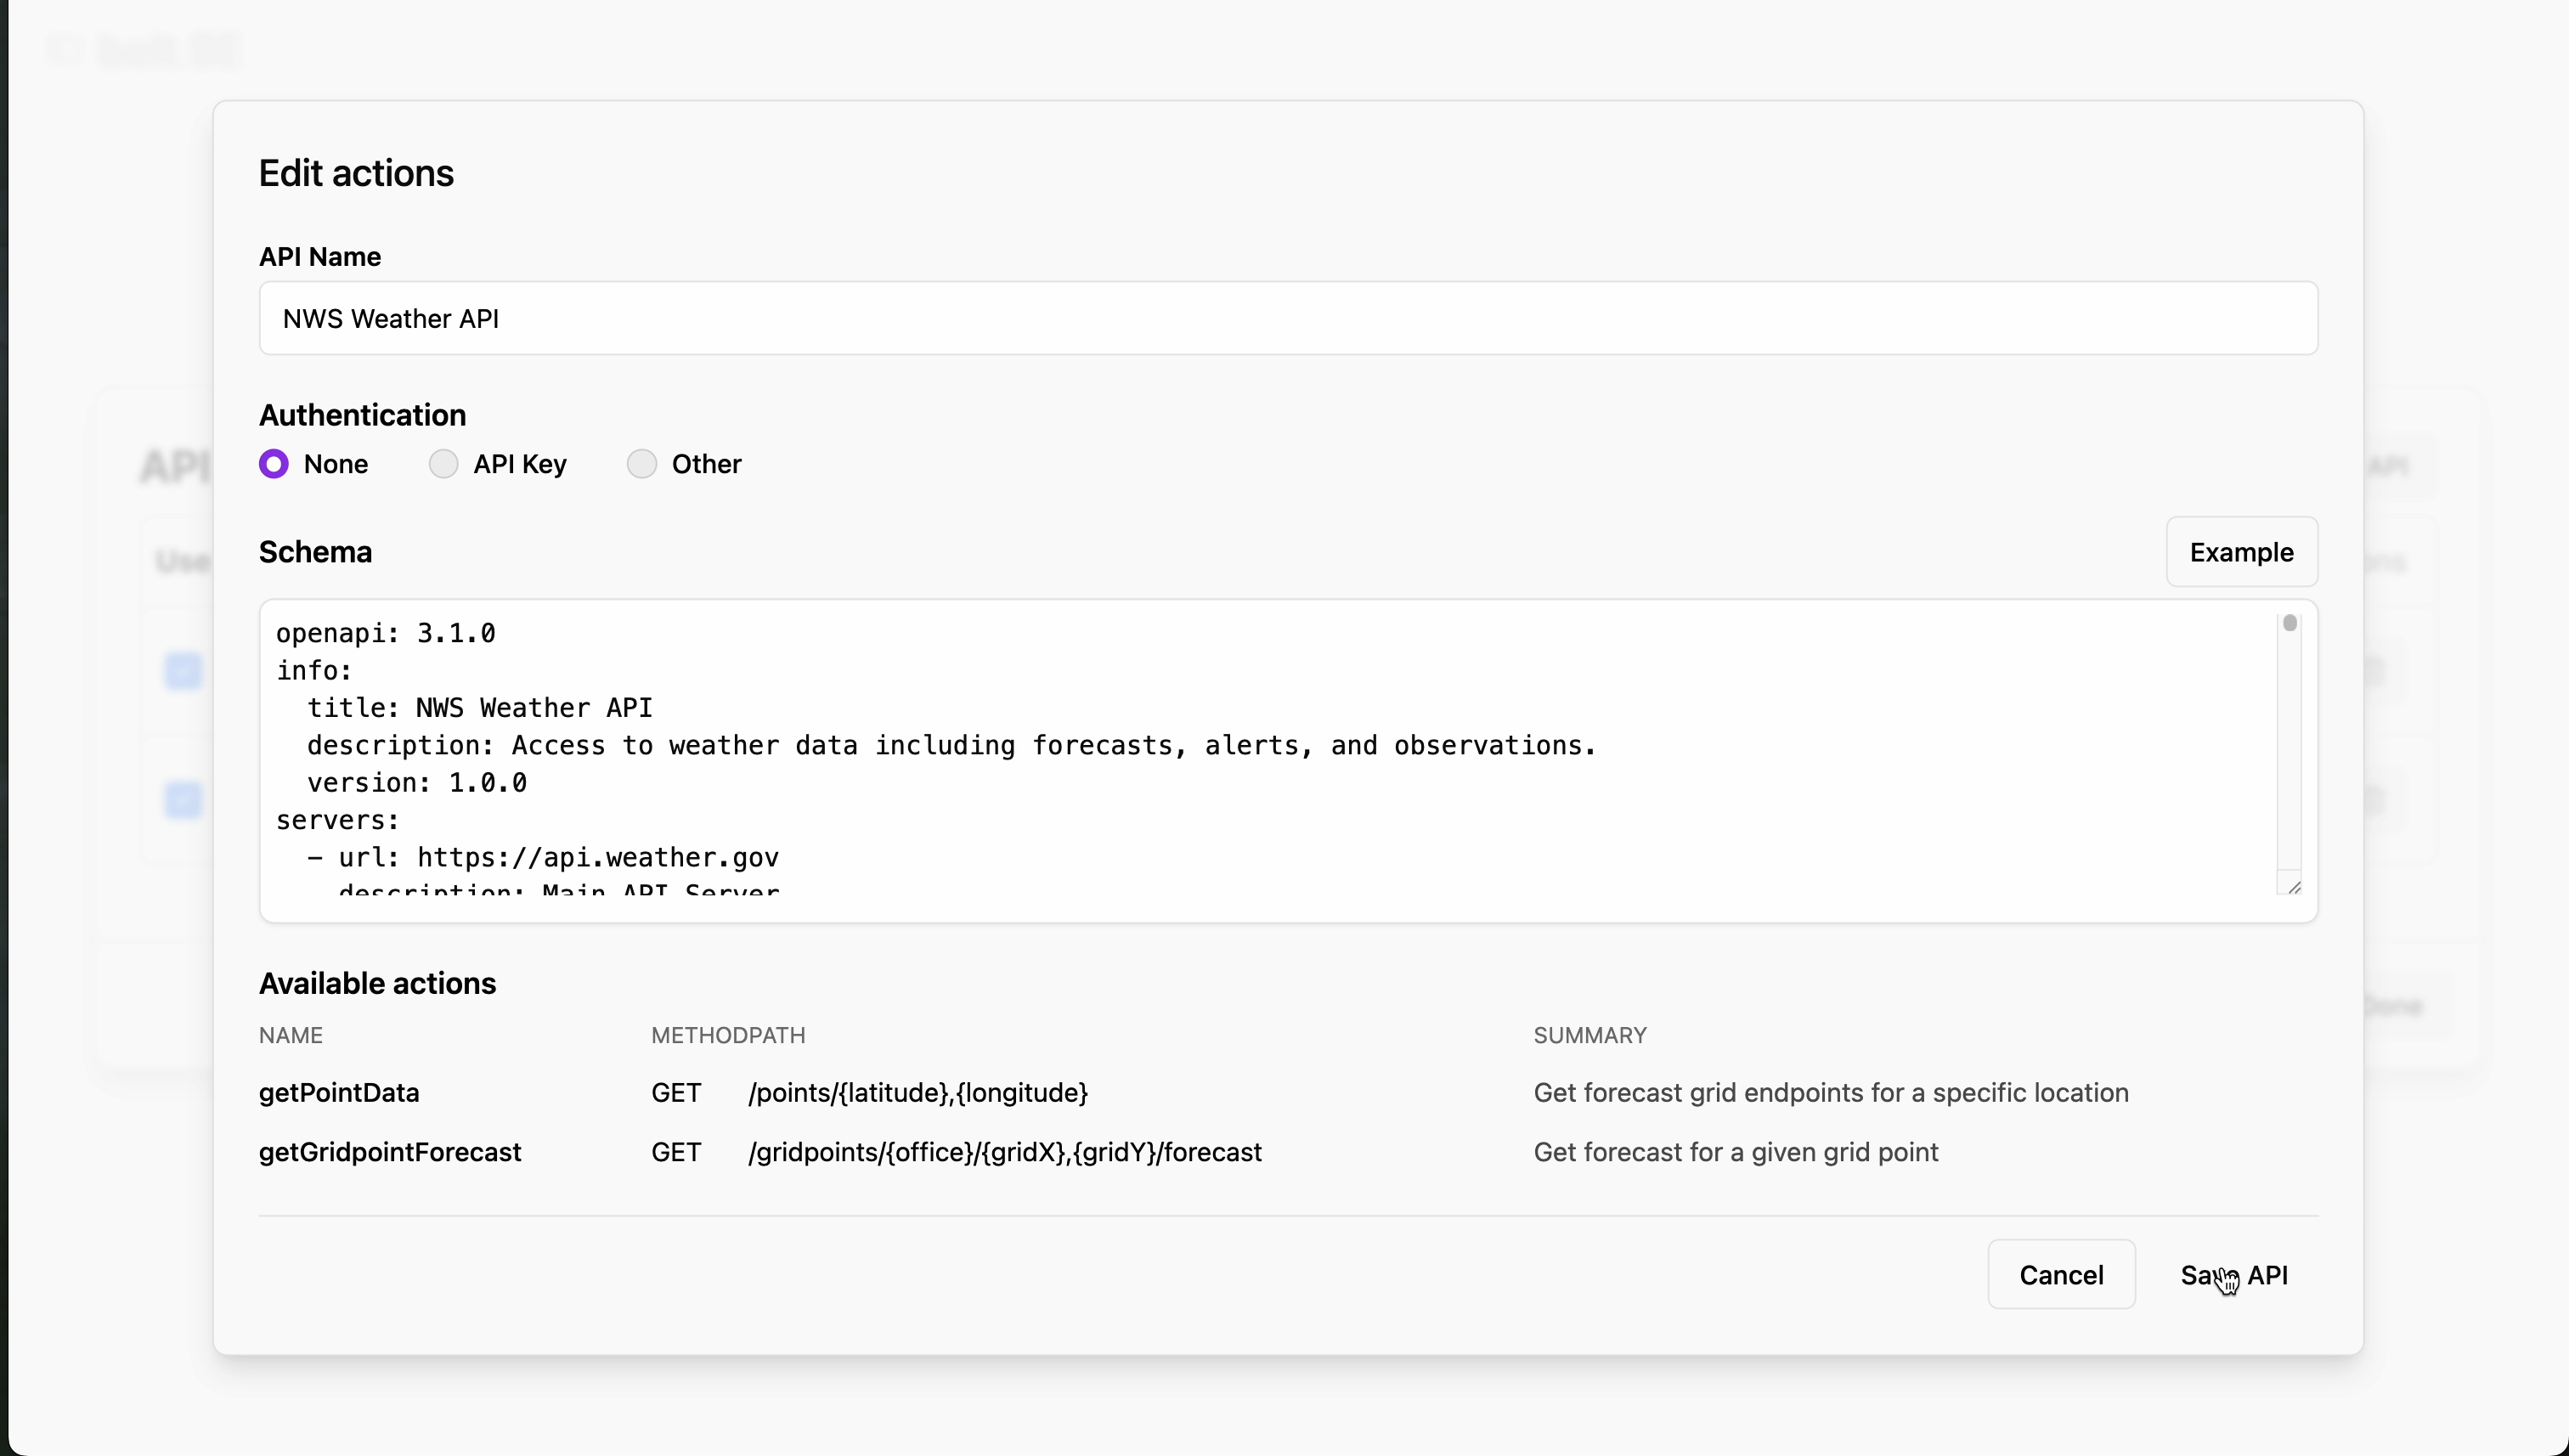
\includegraphics[width=\textwidth]{figures/screenshots/api-actions/demo_edit_modal.png}
  \caption{添加NWS Weather API:粘贴OpenAPI规范定义并配置端点与认证方式}
  \label{fig:demo_edit}
\end{figure}

\begin{figure}[H]
  \centering
  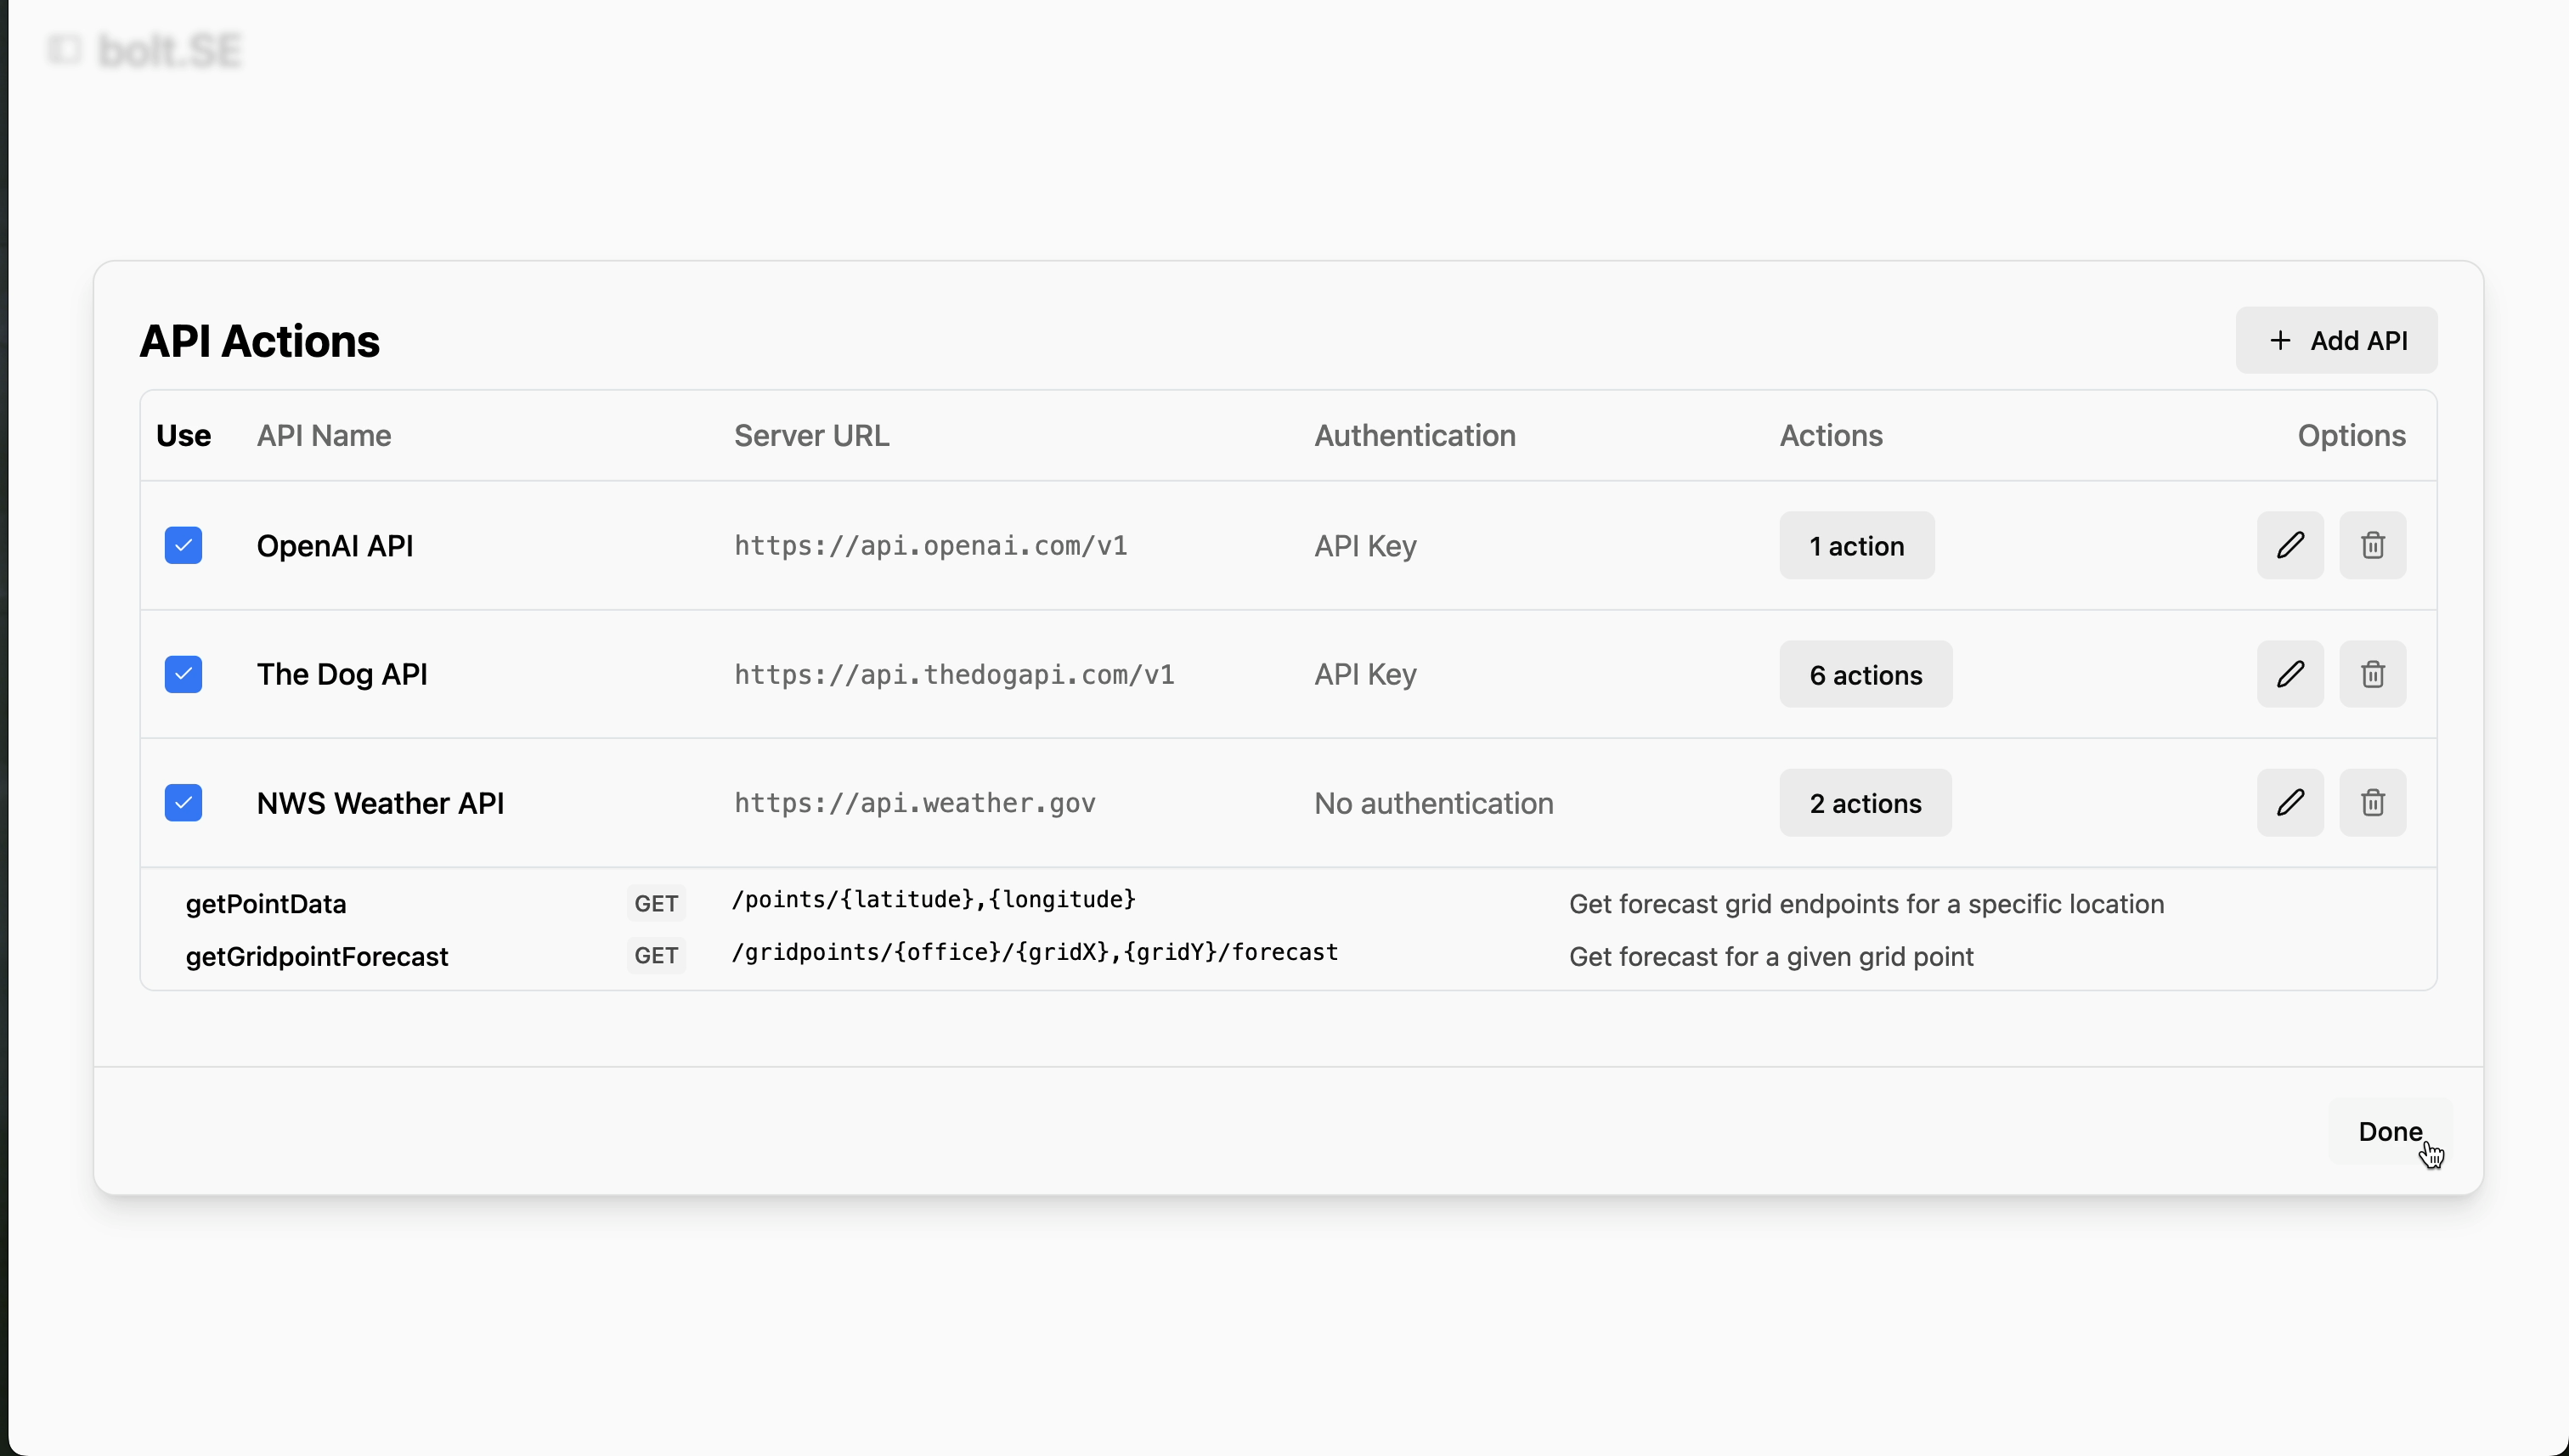
\includegraphics[width=\textwidth]{figures/screenshots/api-actions/demo_actions_table.png}
  \caption{APIActions总览界面:展示所有注册的API、认证方式与可用操作数}
  \label{fig:demo_table}
\end{figure}

\begin{figure}[H]
  \centering
  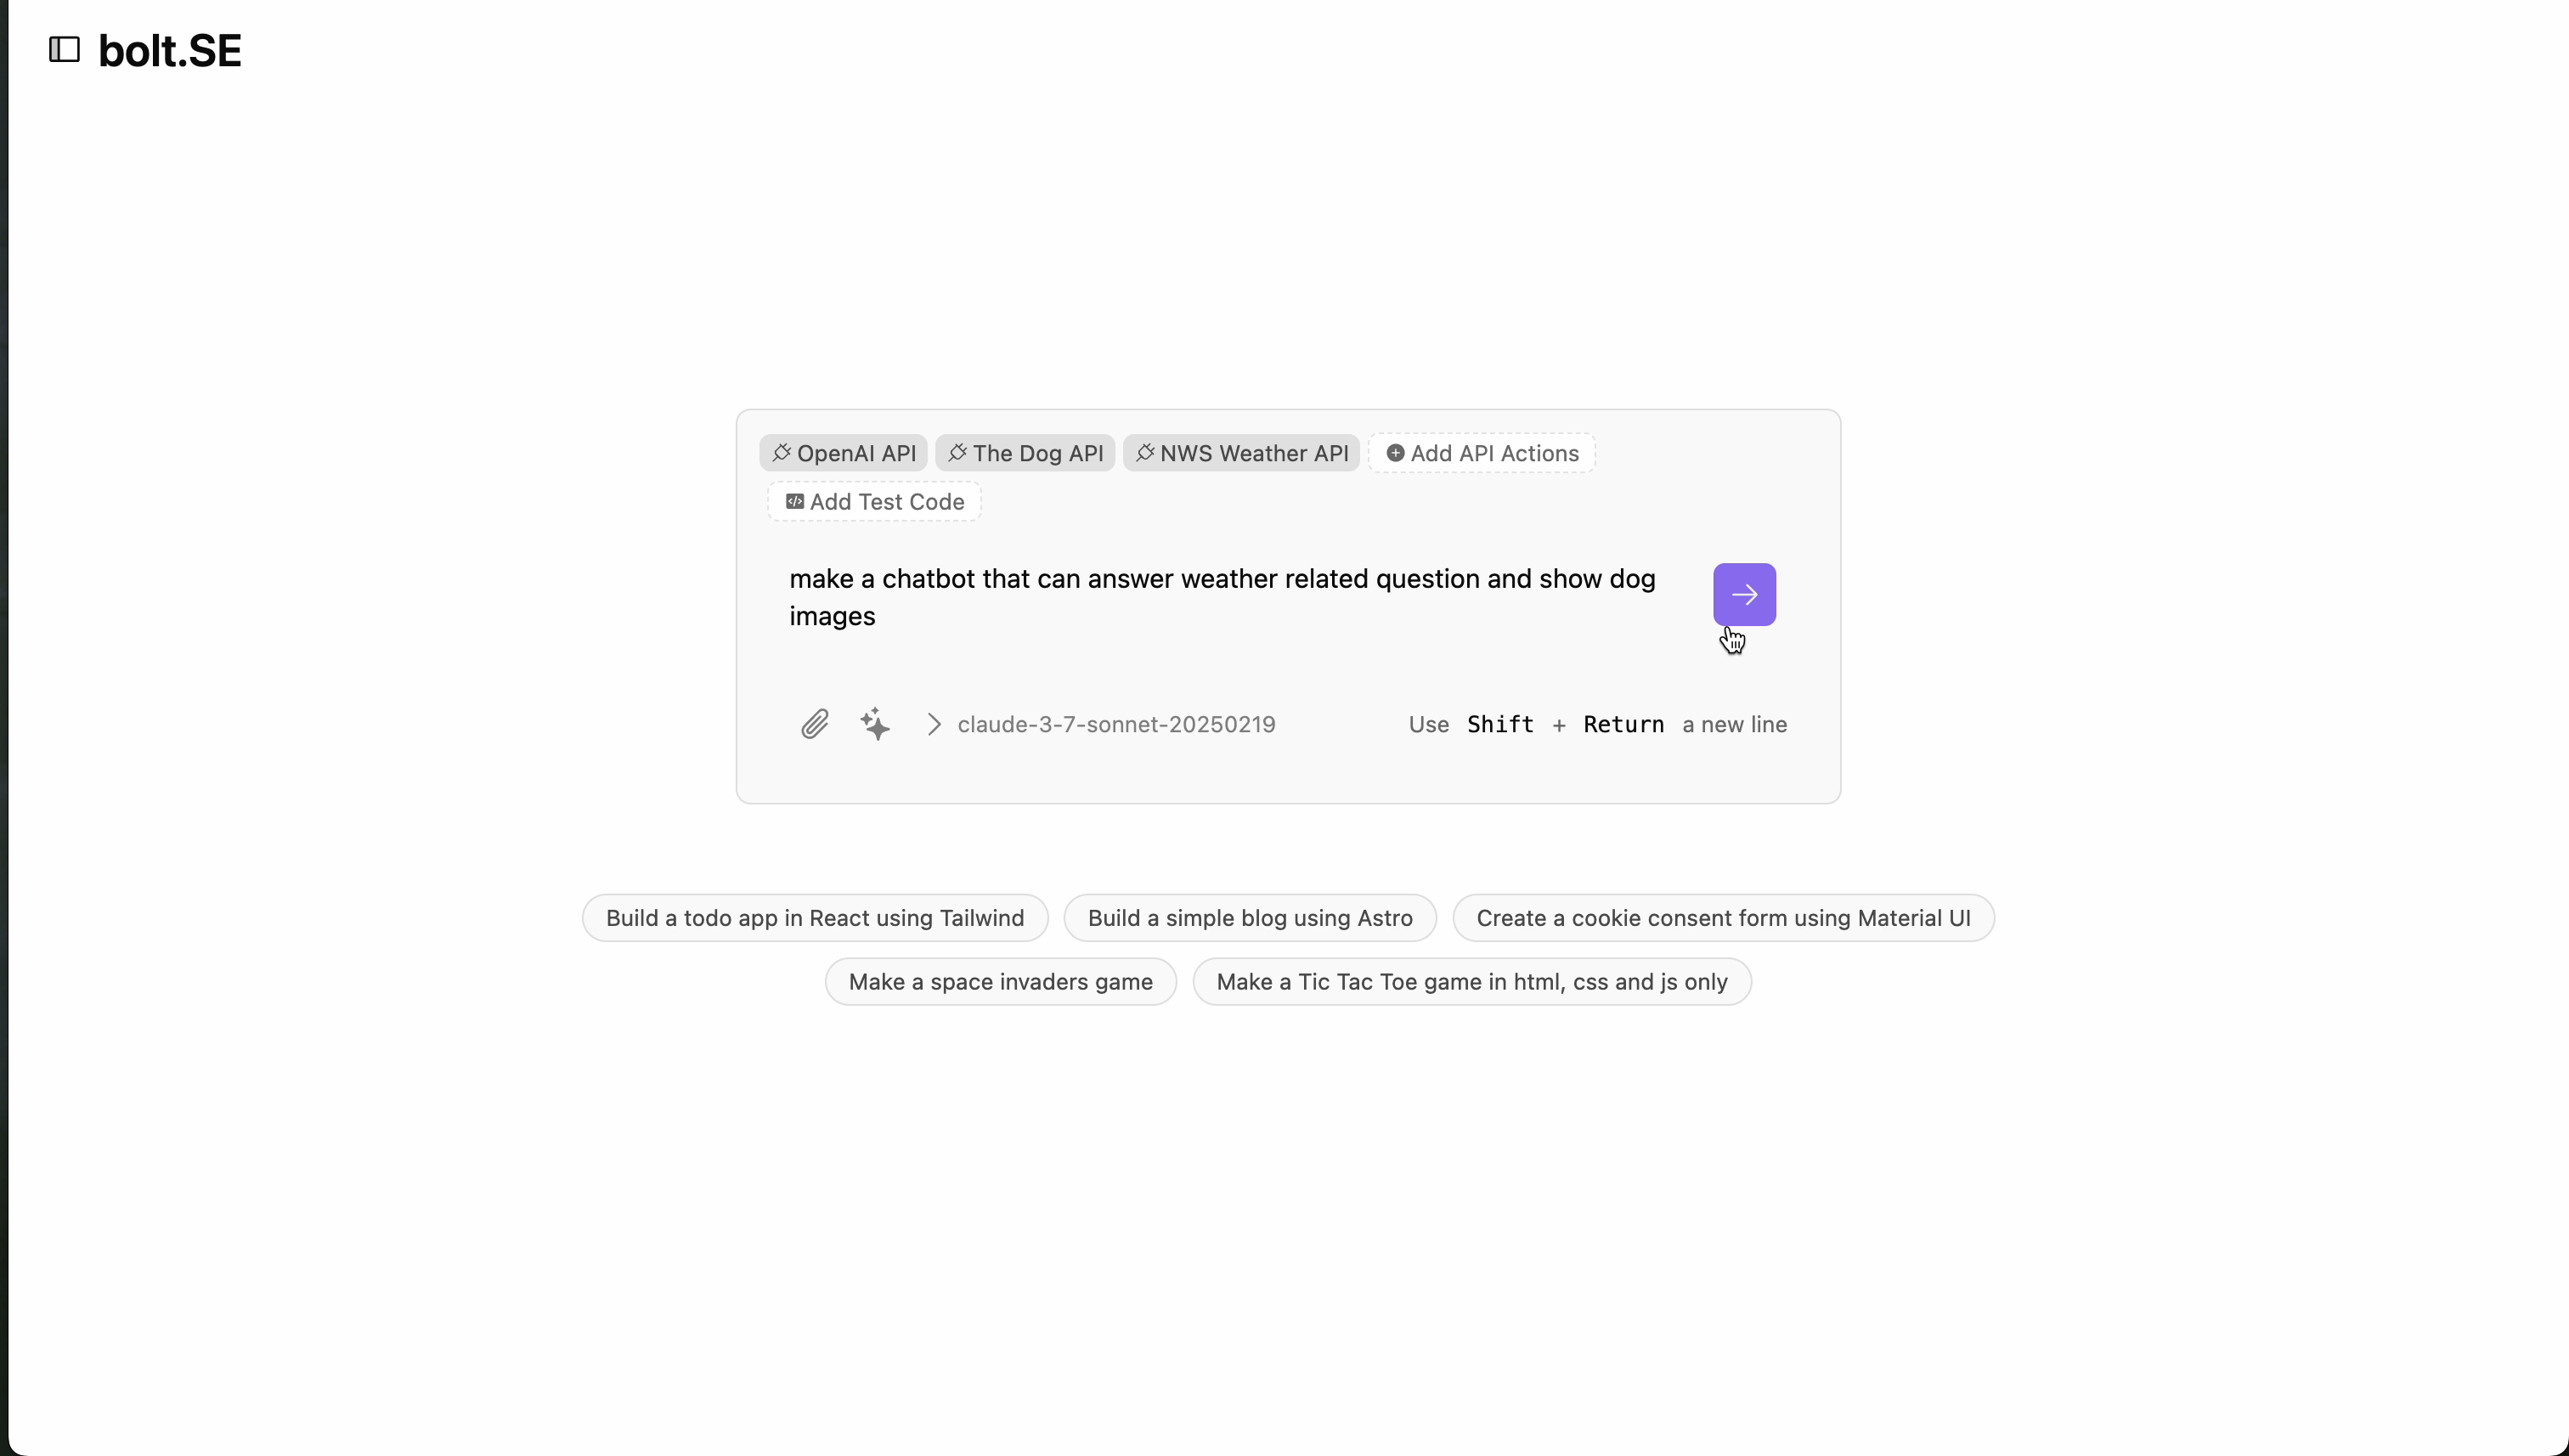
\includegraphics[width=\textwidth]{figures/screenshots/api-actions/demo_prompt_tags.png}
  \caption{对话框中勾选相关API,配合自然语言指令触发任务生成}
  \label{fig:demo_prompt}
\end{figure}

\begin{figure}[H]
  \centering
  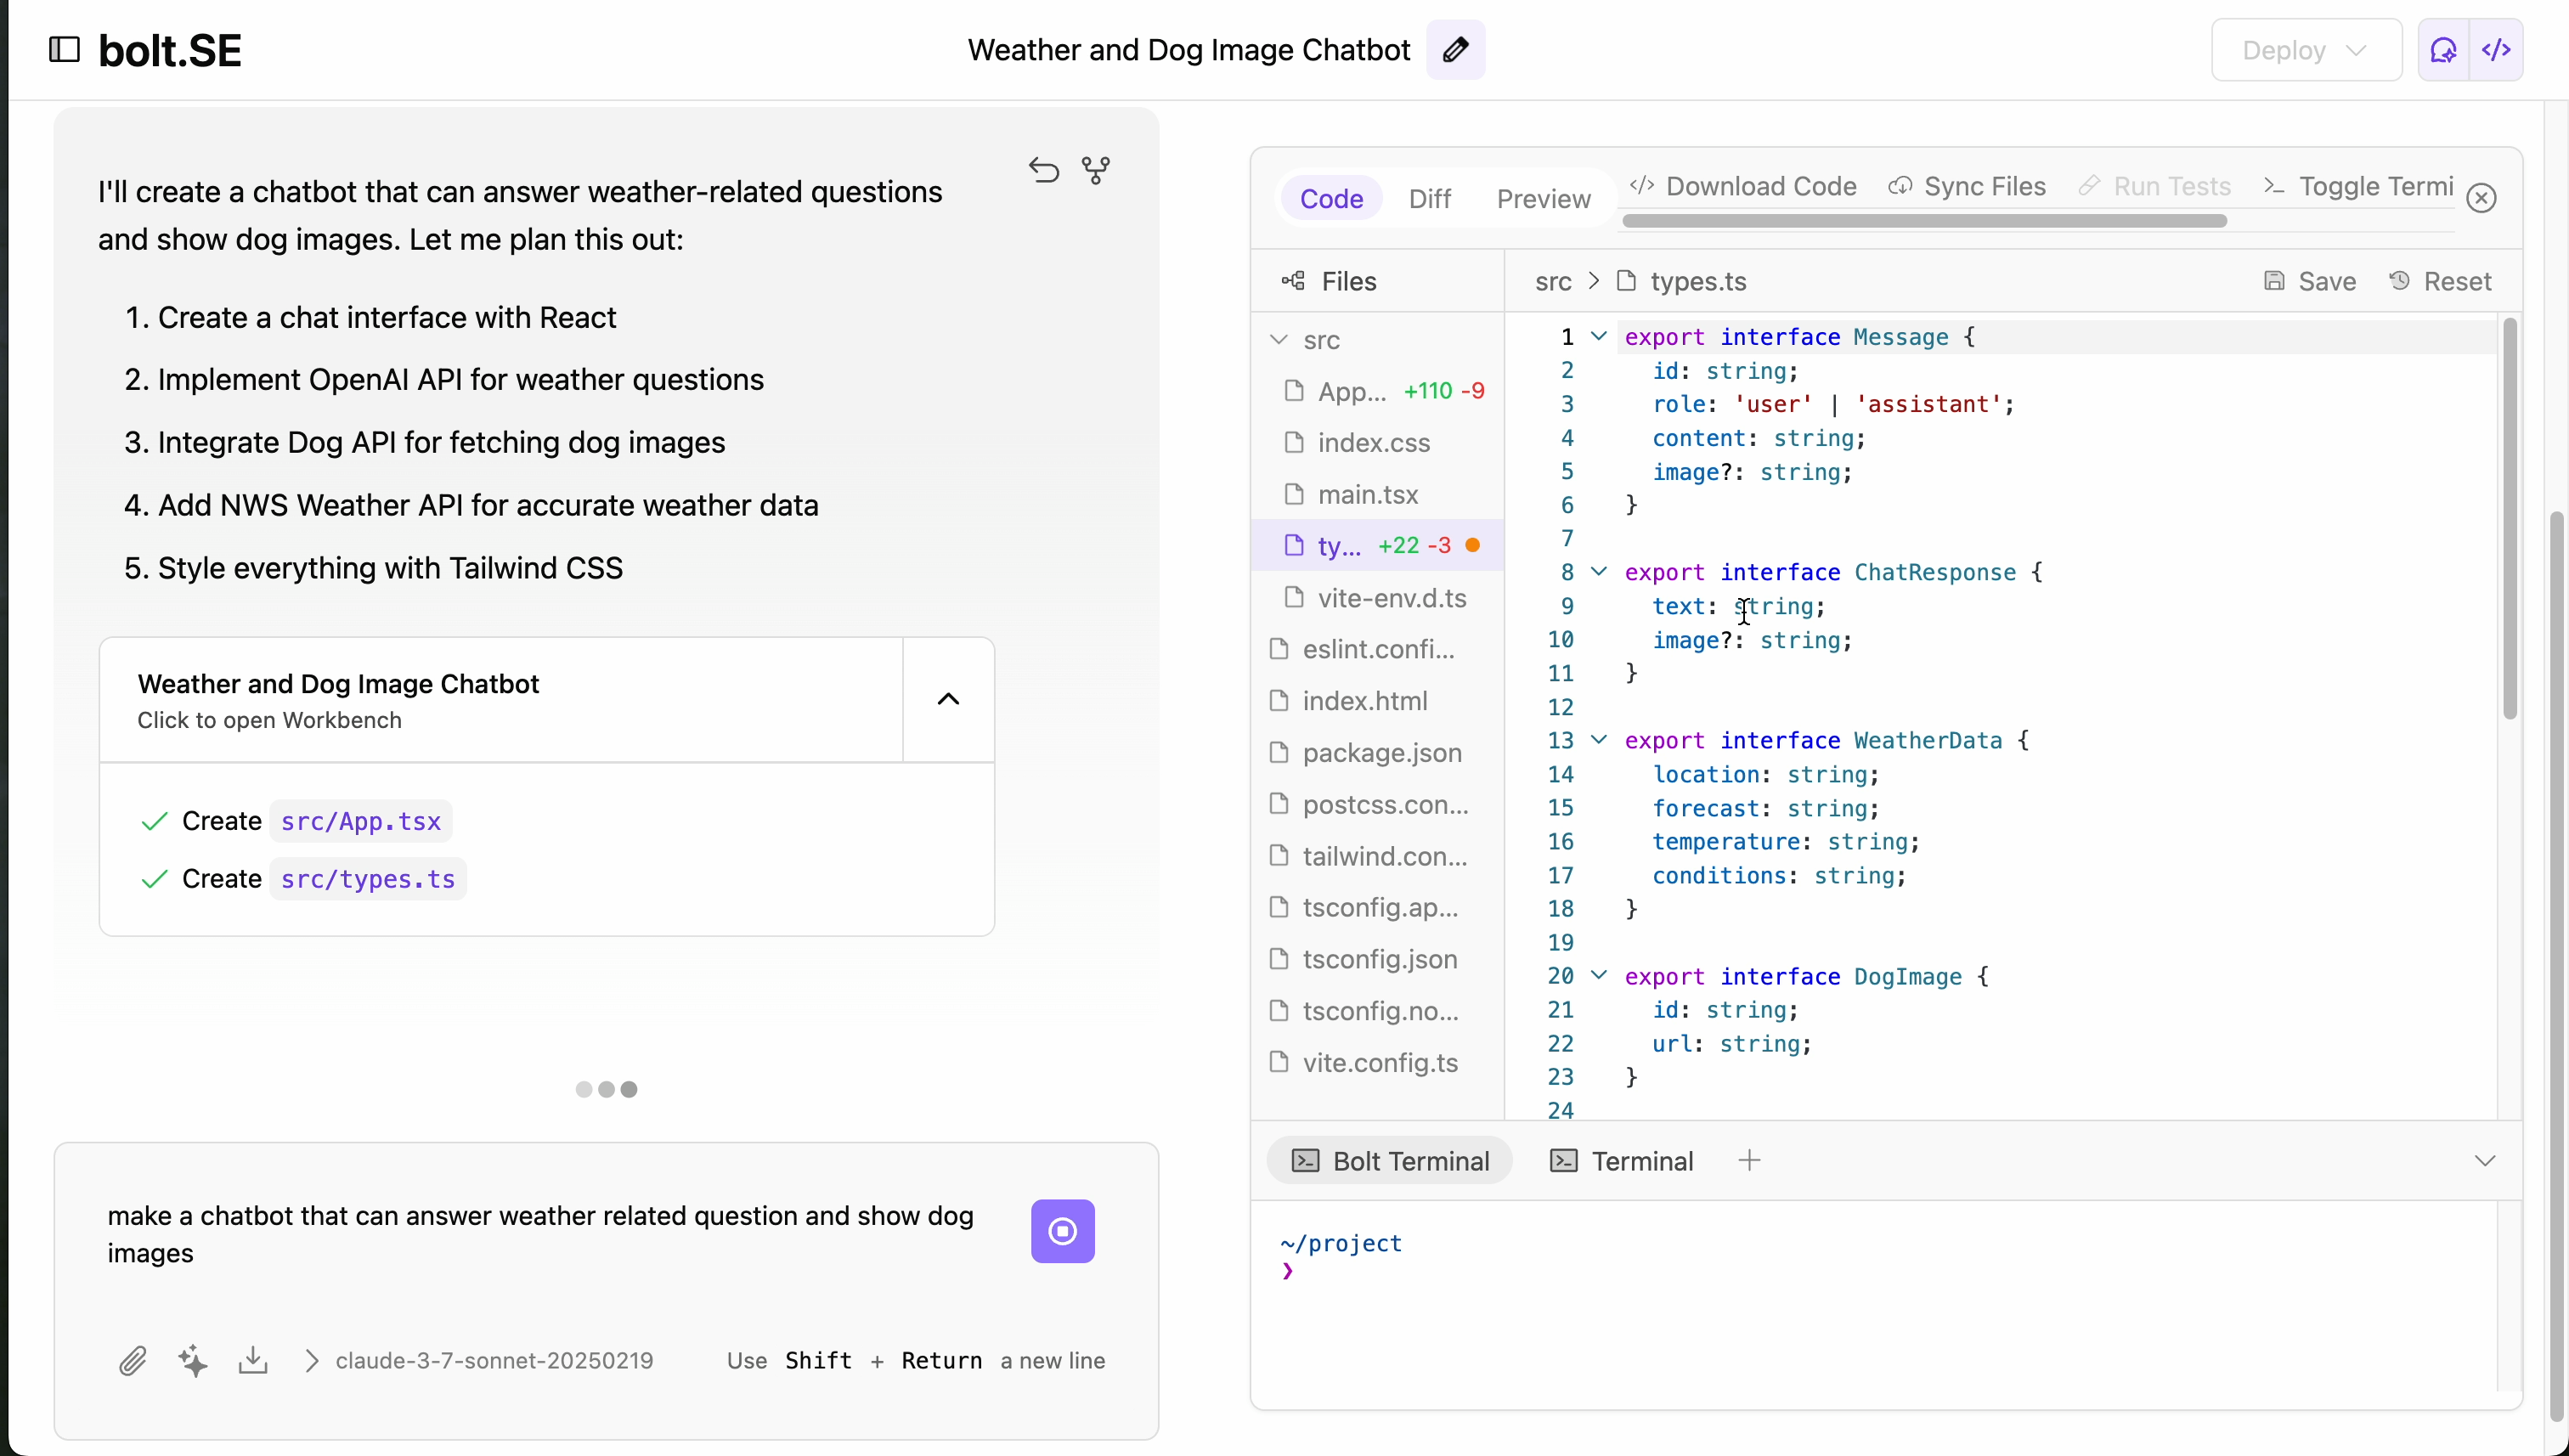
\includegraphics[width=\textwidth]{figures/screenshots/api-actions/demo_plan_files.png}
  \caption{系统生成项目结构与依赖安装命令,包含前端组件与服务调用逻辑}
  \label{fig:demo_plan}
\end{figure}

\subsection{功能验证与效果展示}

在预览界面中,用户可验证机器人能否正确响应请求。如图\ref{fig:demo_dog}所示,用户请求查看狗狗图片时,系统调用The Dog API返回相关图片。图\ref{fig:demo_weather}展示用户询问天气情况时,系统识别意图并调用NWS Weather API提供实时天气信息。这些交互示例展示了APIActions与LLM的协同工作方式,系统能准确理解用户意图并将其转化为相应API调用,体现了API优先开发在LLM应用场景中的实际价值。

\begin{figure}[H]
  \centering
  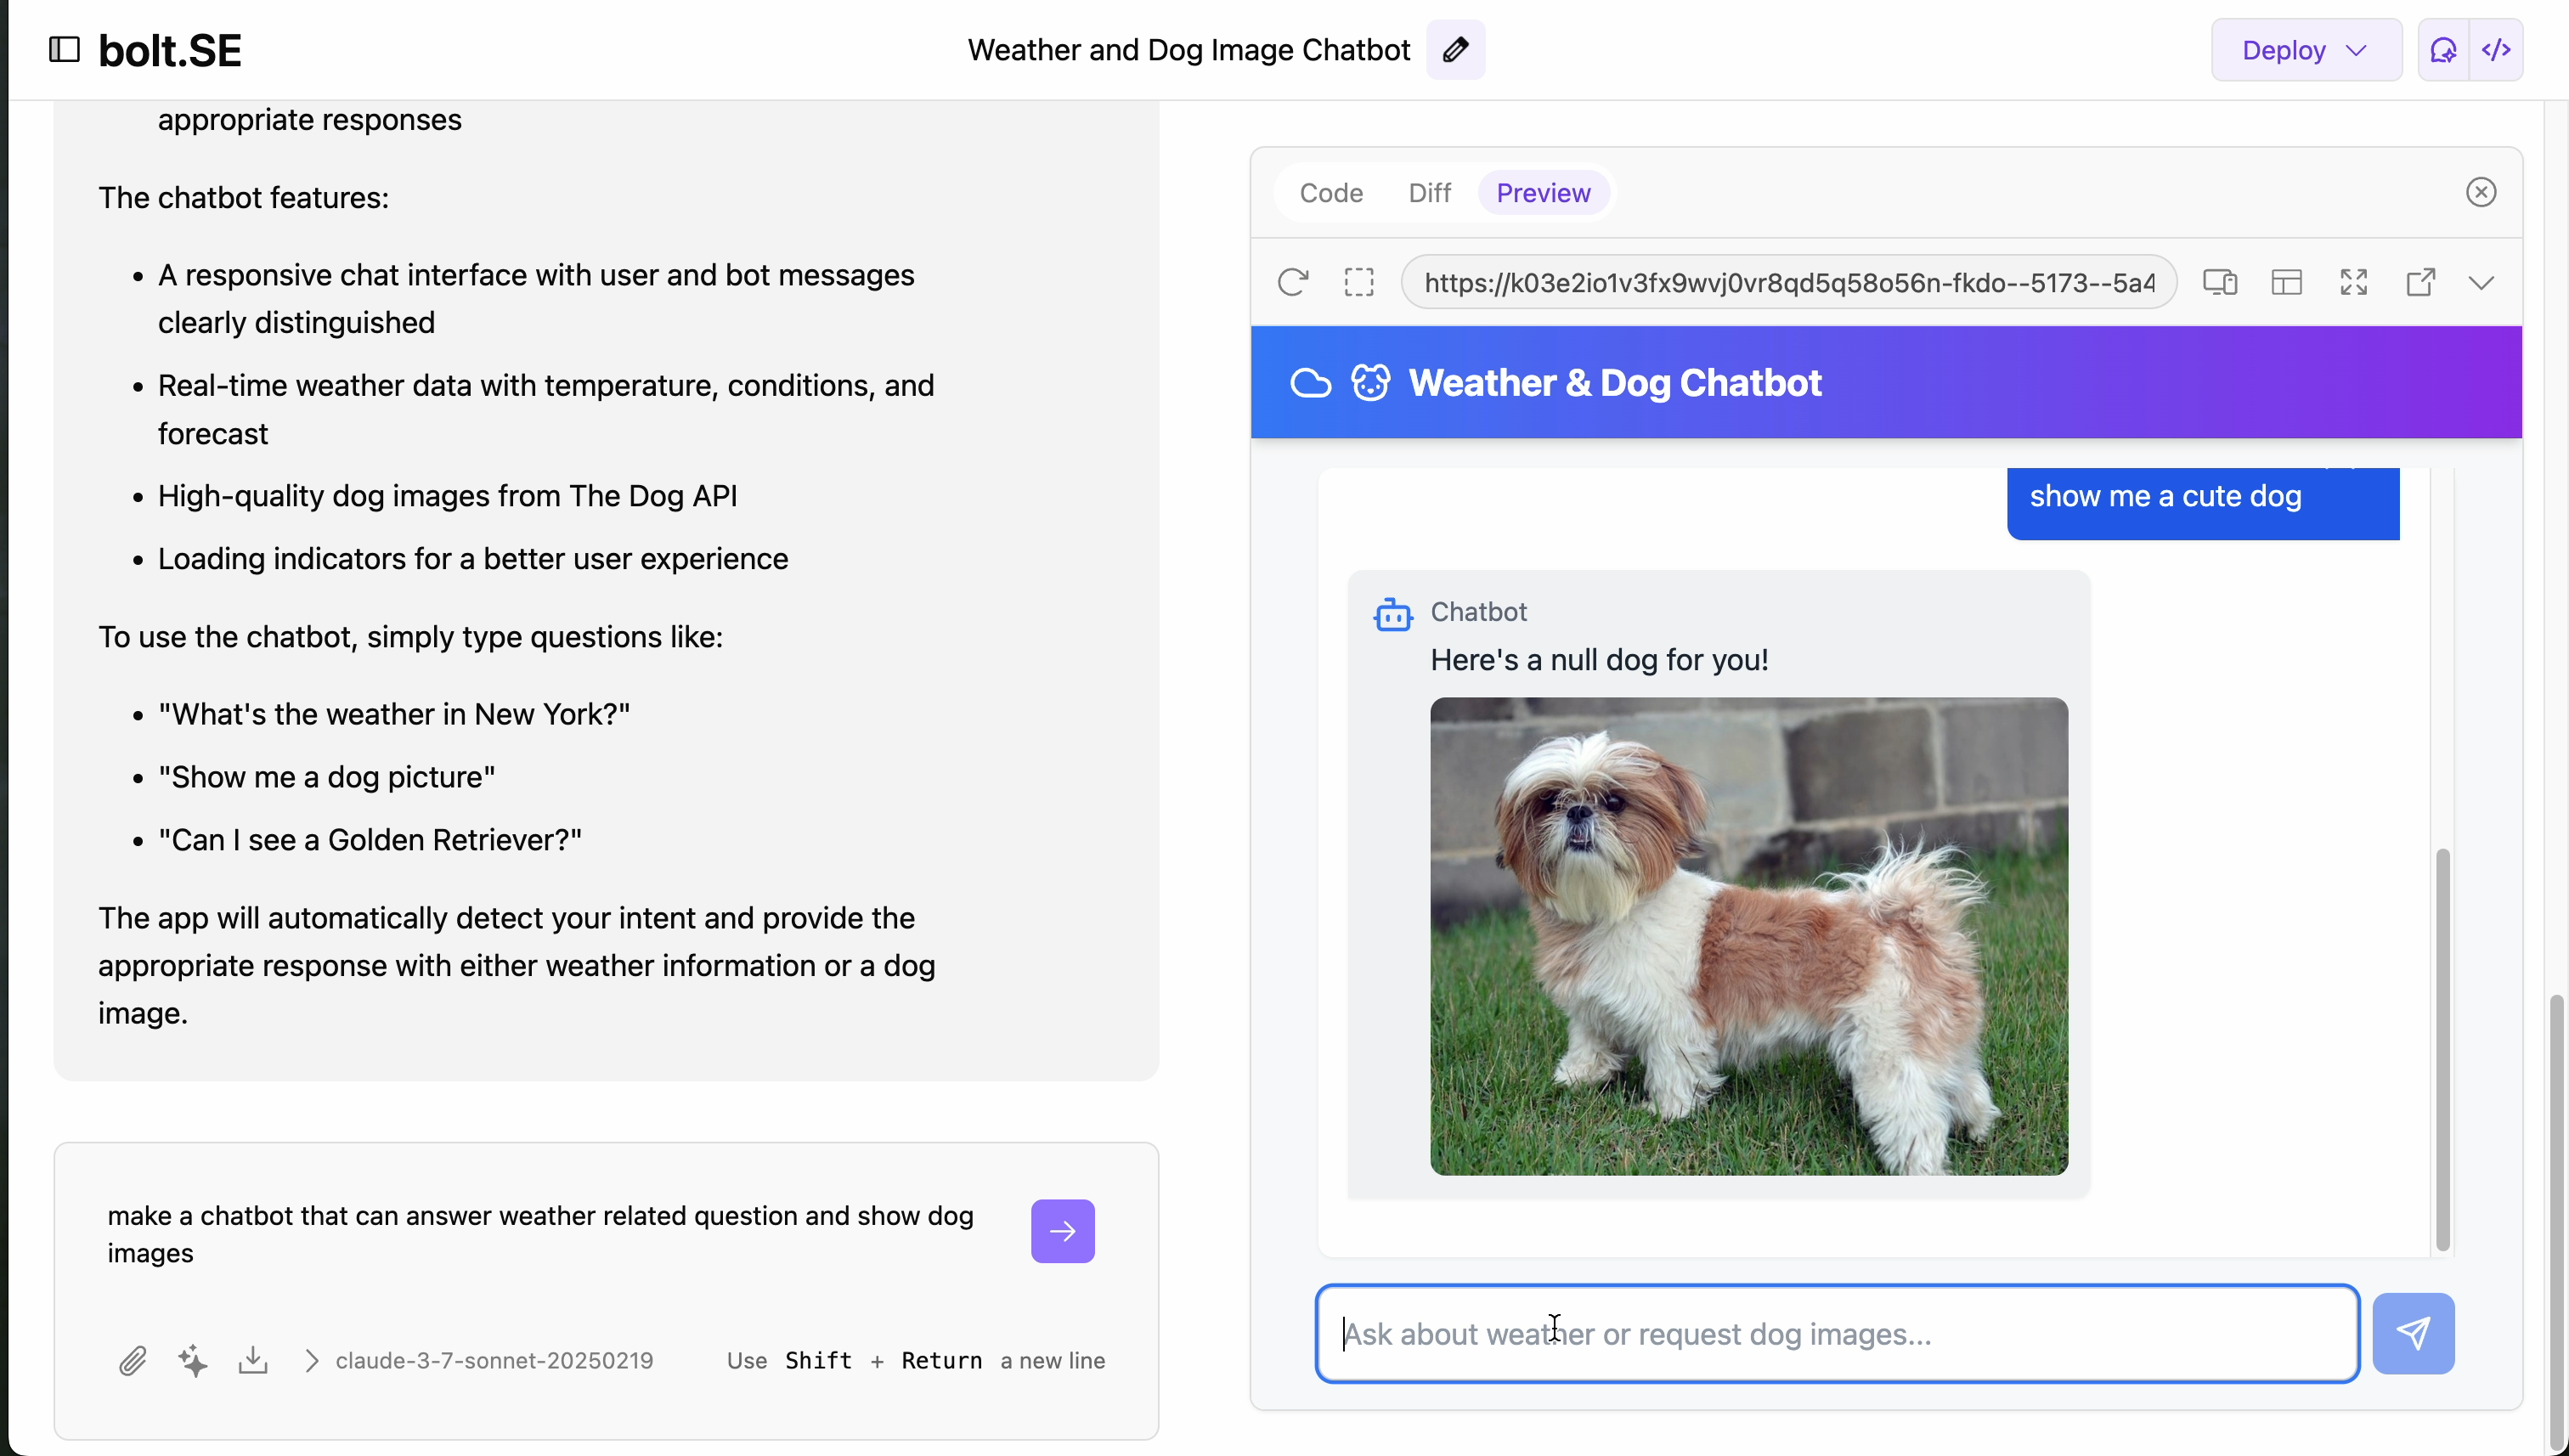
\includegraphics[width=\textwidth]{figures/screenshots/api-actions/demo_dog_preview.png}
  \caption{用户请求"show me a cute dog",系统调用The Dog API返回图片}
  \label{fig:demo_dog}
\end{figure}

\begin{figure}[H]
  \centering
  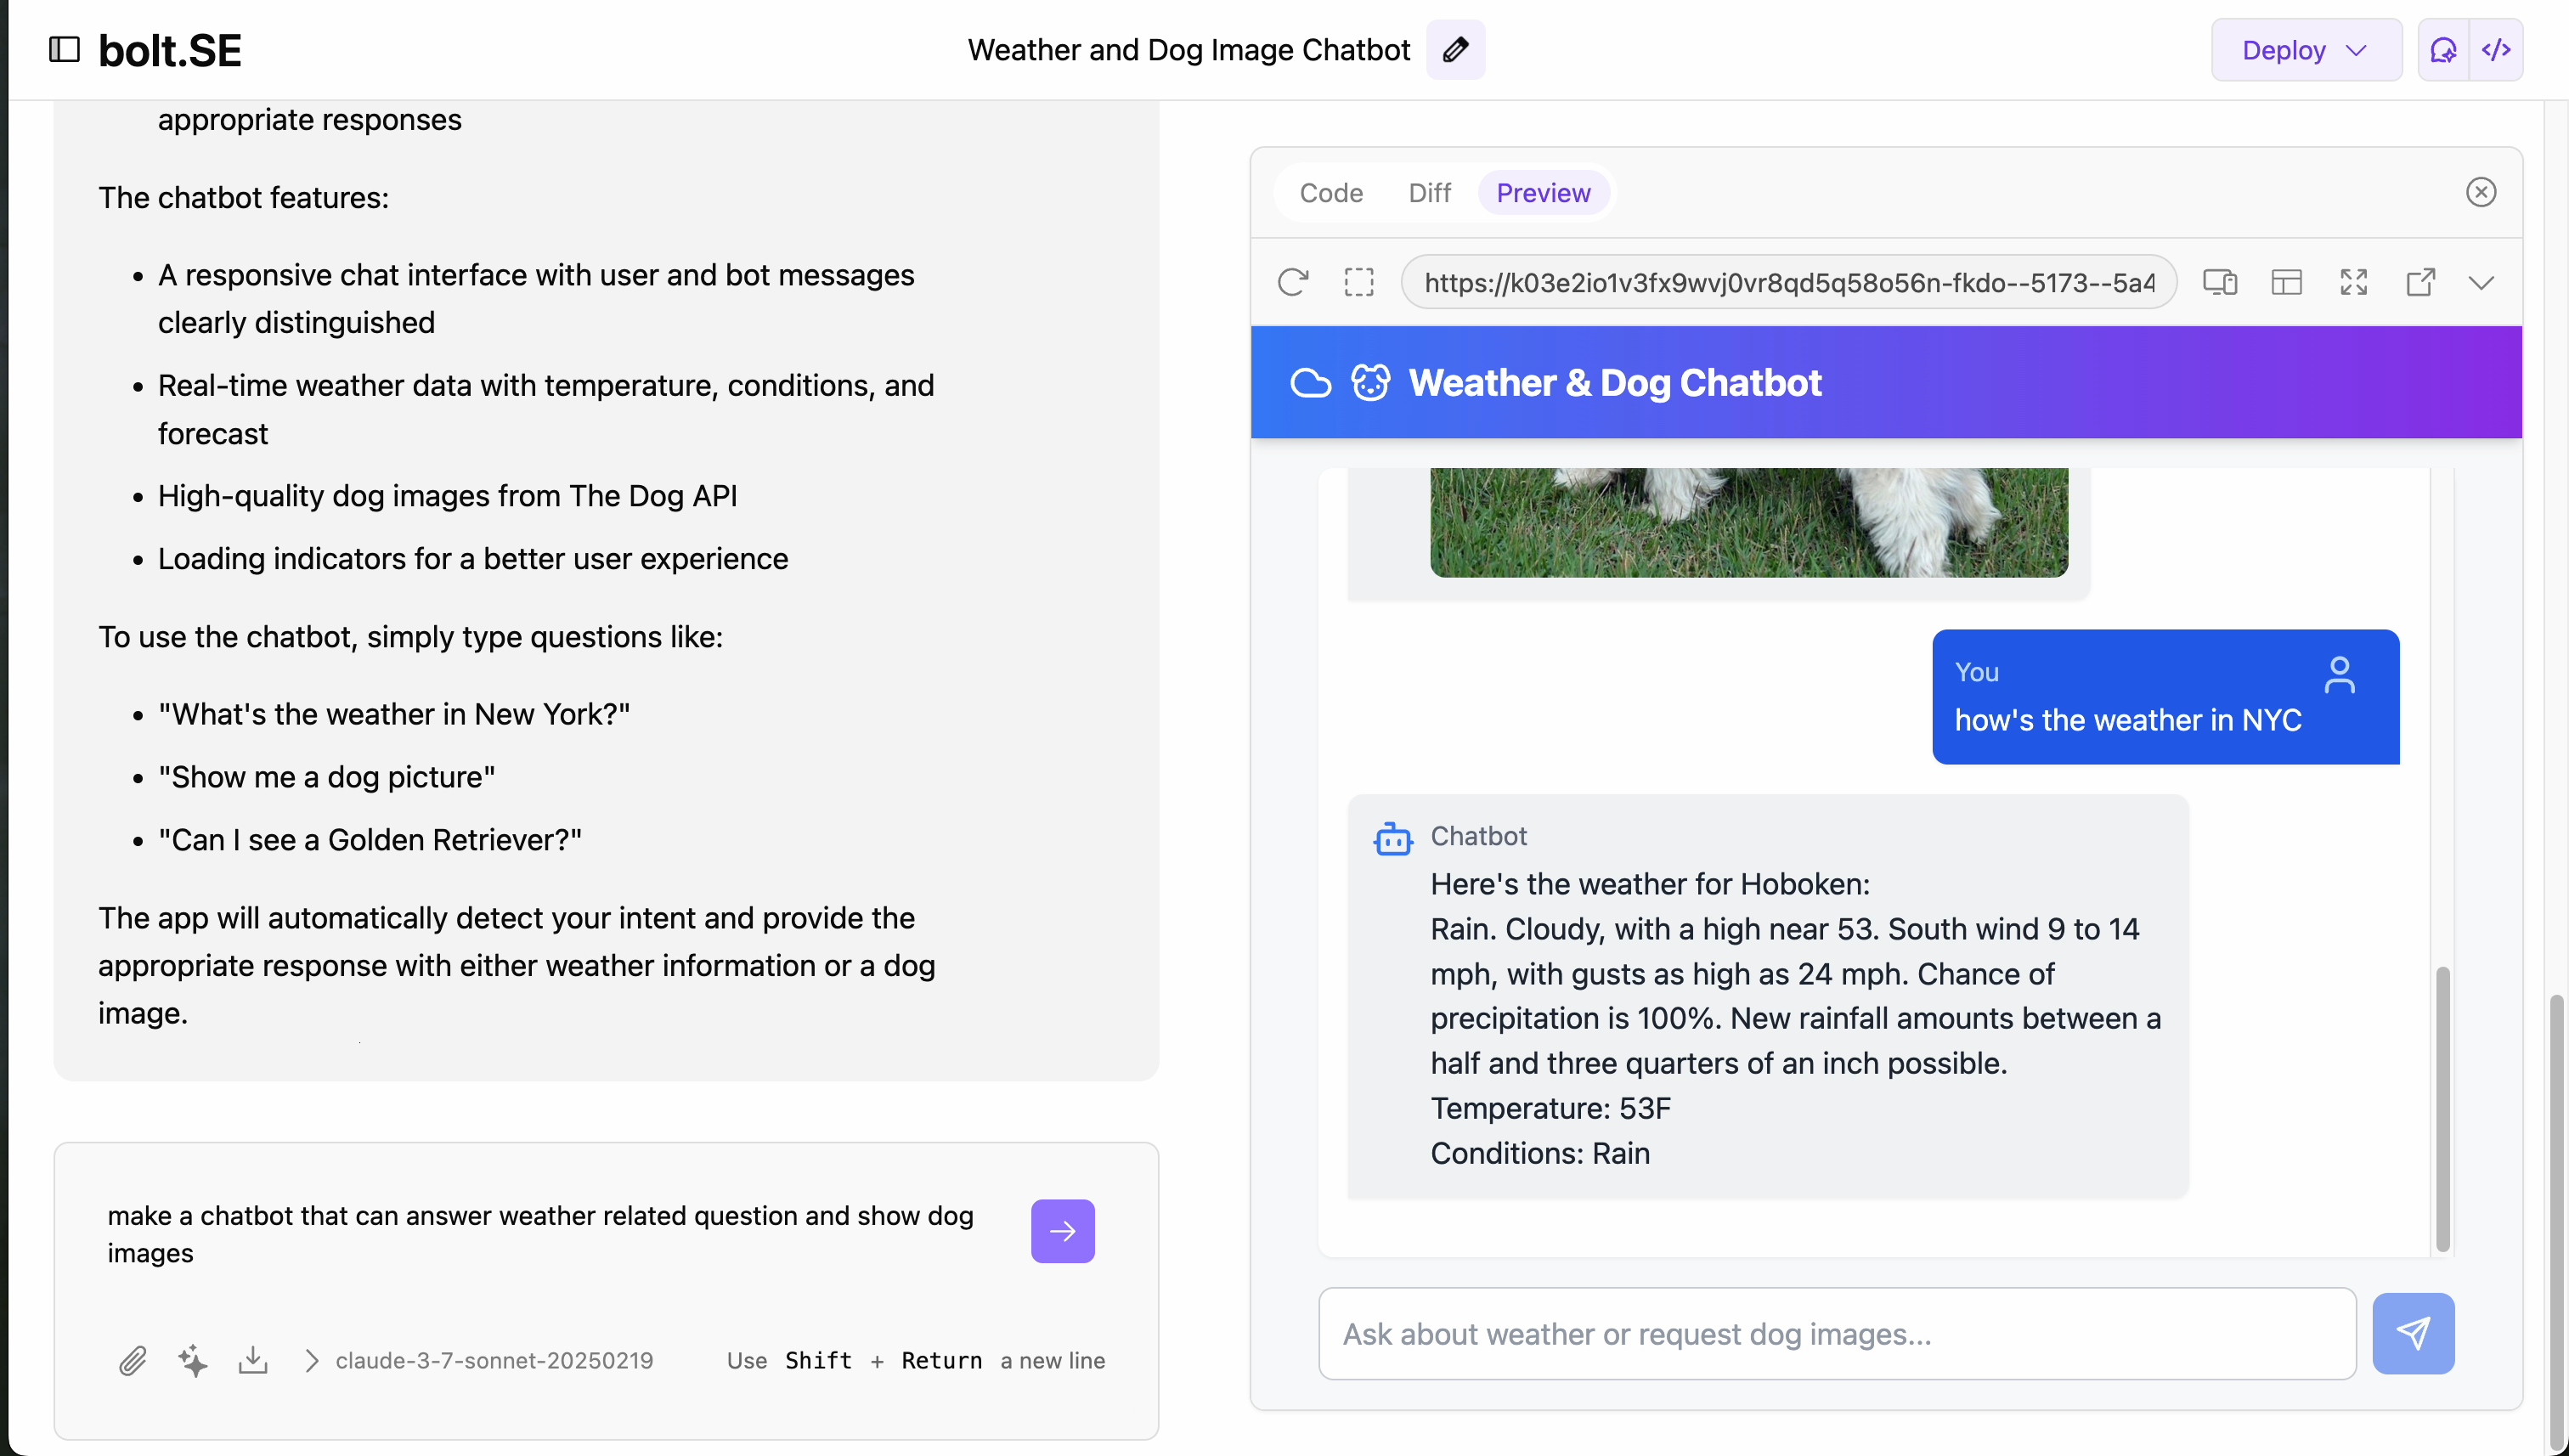
\includegraphics[width=\textwidth]{figures/screenshots/api-actions/demo_weather_preview.png}
  \caption{询问天气时,系统识别意图并调用NWS Weather API提供实时天气信息}
  \label{fig:demo_weather}
\end{figure}